\section{Auswertung}
\label{sec:Auswertung}
\subsection{Bestimmung des \texorpdfstring{\textsc{Planck}}{Planck}schen Wirkungsquantum}
Die Messwerte sind in Tabelle \ref{tab:messwerte} aufgetragen.
In Abbildungen \ref{fig:uidiagramm1} bis \ref{fig:uidiagramm2} sind die gemessenen Bremsspannungen $U_\text{B}$ gegen die Wurzel des Photostroms $I_0$ aufgetragen.
Die Parameter für die Ausgleichsgeraden werden nach den Formeln \eqref{eq:regress}
\begin{figure}[p]
\centering
Regression nach
\begin{subequations}
	\begin{equation}
		\Delta = N \sum{x^2} - {\biggl(\sum{x}\biggr)}^2,
	\end{equation}
	\begin{equation}
		a_{\text{Reg}} = \frac{N\sum{x\cdot y} - \sum{x} \cdot \sum{y}}{\Delta},
	\end{equation}
    \begin{equation}
		b_{\text{Reg}} = \frac{\sum{x^2} \cdot \sum{y} - \sum{x} \cdot \sum{x \cdot y}}{\Delta},
	\end{equation}
	\begin{equation}
		\sigma_{y} = \sqrt{\frac{\sum{(y - a_{\text{Reg}} \cdot x - b_{\text{Reg}})^2}}{N - 2}},
	\end{equation}
	\begin{equation}
		\sigma_{a} = \sigma_{y} \sqrt{\frac{N}{\Delta}},
	\end{equation}
	\begin{equation}
		\sigma_{b} = \sigma_{y} \sqrt{\frac{\sum{x^2}}{\Delta}}
	\end{equation}
	mit $x=x_\text{lin}=\frac{1}{T_m^2}$, $y=B$, $a_\text{Reg}=a_\text{lin}$, $b_\text{Reg}=b_\text{lin}$ und der Anzahl der Datenpaare N.
	\label{eq:regress}
\end{subequations}
\end{figure}
bestimmt.\\
Es ergeben sich die Fitparameter
\begin{table}
	\centering
	\begin{tabular}{l S[table-format=3] S[table-format=1.2] S[table-format=1.2]}
		\toprule
		\multicolumn{2}{c}{Lichtspektrallinie} &\multicolumn{2}{c}{Fitparameter} \\
		{Farbe} & {Wellenlänge/$\:\si{\nano\meter}$} &{Steigung$/\:\si{\volt\per{\nano\meter}}$} & {Abschnitt$/\:\si{\volt}$}\\
		\midrule
			{rot} 		&640	&-0.25  &0.77\\
			{gelb} 		&578	&-0.04  &0.34\\
			{grün} 		&546	&-0.03  &0.44\\
			{violett}	&435.8	&-0.04  &0.91\\
			{ultraviolett} &366	&-0.08  &1.47\\
		\bottomrule
	\end{tabular}
	\caption{Fitparameter der \texorpdfstring{Abbildungen \ref{fig:uidiagramm1} bis \ref{fig:uidiagramm2}}{U-I-Diagramme}}
	\label{label}
\end{table}

Weiter werden die y-Achsenabschnitte der Fits gegen die Lichtfrequenz $\nu$ in Abbildung \ref{fig:unu} aufgetragen. 
Für die Umrechnung von Wellenlänge $\lambda$ und $\nu$ gilt
\begin{equation}
	c_0=\lambda\cdot\nu.
\end{equation}

Gemäß der \textsc{Einstein}schen Formel \eqref{eq:einstein}
\begin{align}
	%E_\text{kin.} &= e\cdot U = {h}\cdot{\nu} - {W_\text{A}}\\
	\underbrace{U}_{y_\text{lin}} &= \underbrace{\frac{h}{e}}_{a_\text{lin}}\cdot\underbrace{\nu}_{x_\text{lin}} - \underbrace{\frac{W_\text{A}}{e}}_{b_\text{lin}}\\
\end{align}
werden aus den Fitparametern das Plancksche Wirkungsquantum und die Austrittsarbeit bestimmt.

Es folgt
\begin{alignat}{3}
	\frac{h}{e}=\SI{3.38(64)e-15}{\weber} \quad&\text{und} \quad&&\frac{W_\text{A}}{e}= \SI{-1.41(36)}{\volt}.
\end{alignat}



\begin{figure}[p]
	\centering
	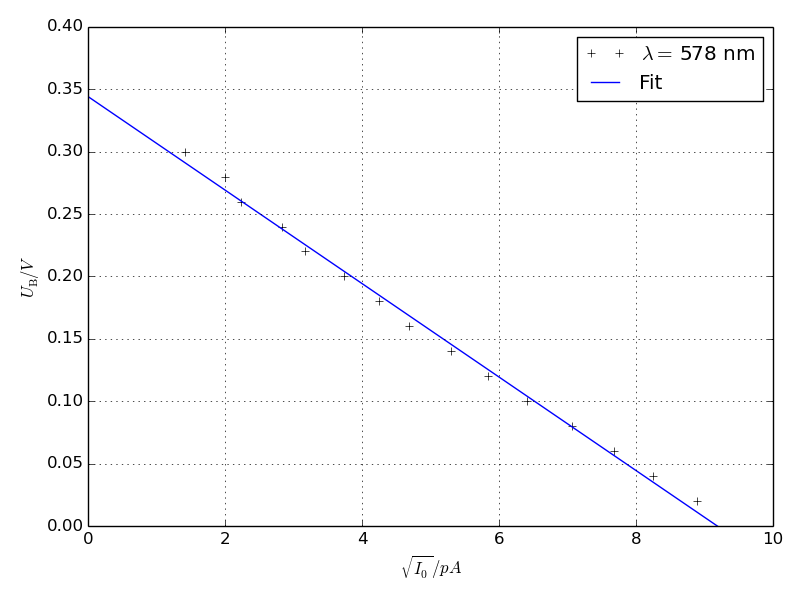
\includegraphics[width=0.8\textwidth]{Bilder/Fit_gelb.png}
	\caption{Gemessene Photostromstärken in Abhängigkeit von den Bremsspannungen, Messung bei gelber Spektrallinie.}
	\label{fig:uidiagramm1}
\end{figure}
\begin{figure}[p]
	\centering
	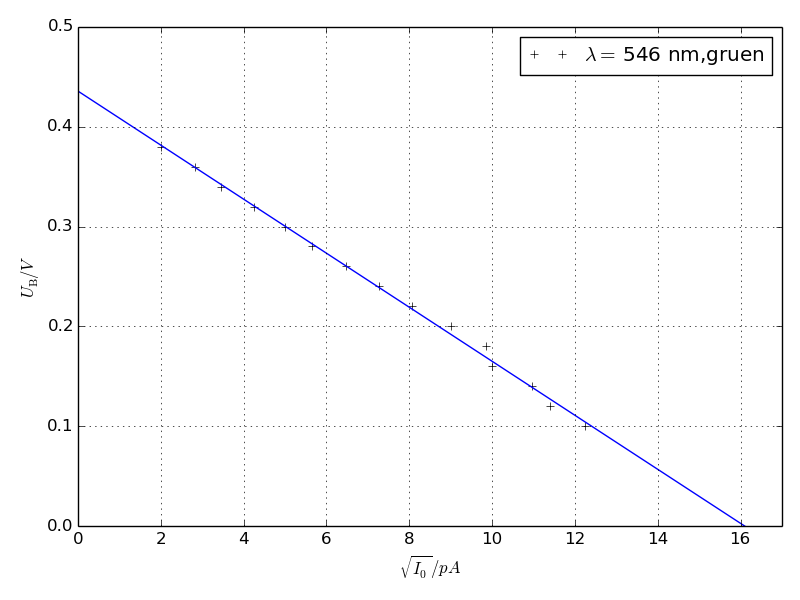
\includegraphics[width=0.8\textwidth]{Bilder/Fit_gruen.png}
	\caption{Gemessene Photostromstärken in Abhängigkeit von den Bremsspannungen, Messung bei grüner Spektrallinie.}
\end{figure}
\begin{figure}[p]
	\centering
	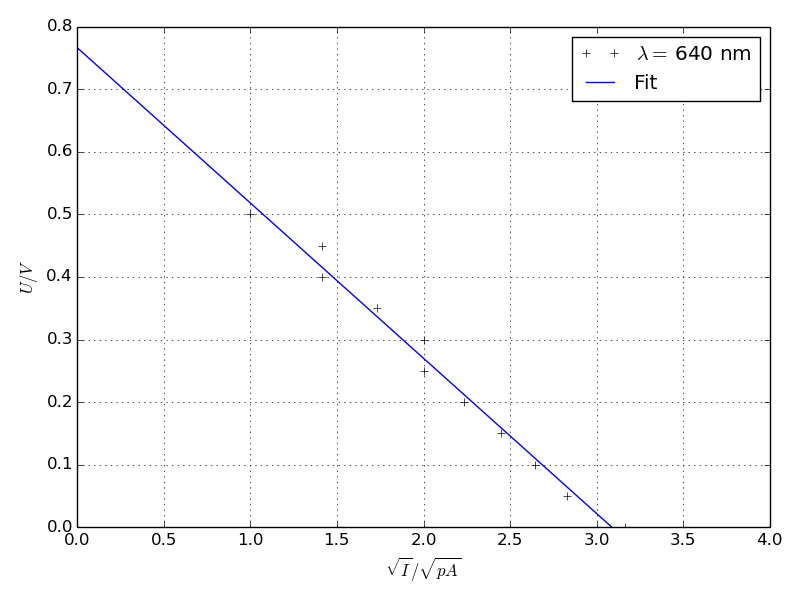
\includegraphics[width=0.8\textwidth]{Bilder/Fit_rot.png}
	\caption{Gemessene Photostromstärken in Abhängigkeit von den Bremsspannungen, Messung bei roter Spektrallinie.}
\end{figure}
\begin{figure}[p]
	\centering
	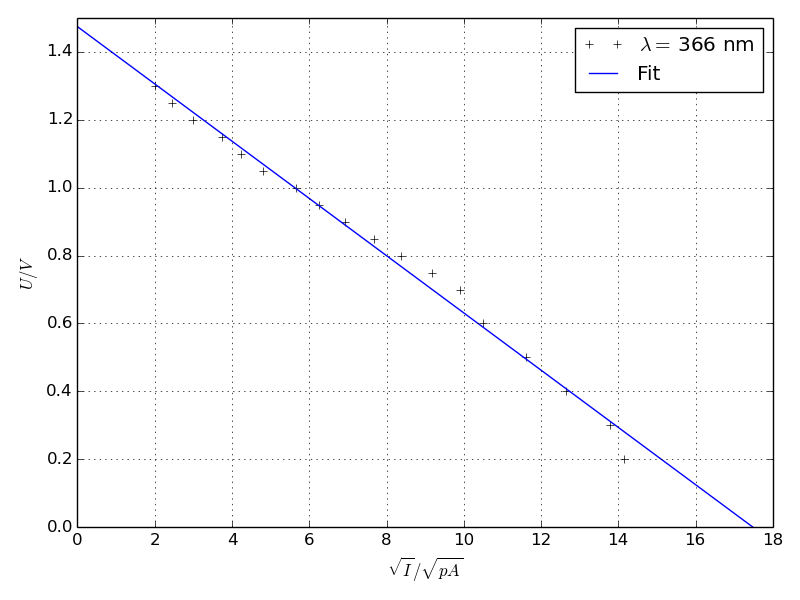
\includegraphics[width=0.8\textwidth]{Bilder/Fit_uv.png}
	\caption{Gemessene Photostromstärken in Abhängigkeit von den Bremsspannungen, Messung bei UV-Spektrallinie.}
\end{figure}
\begin{figure}[pt]
	\centering
	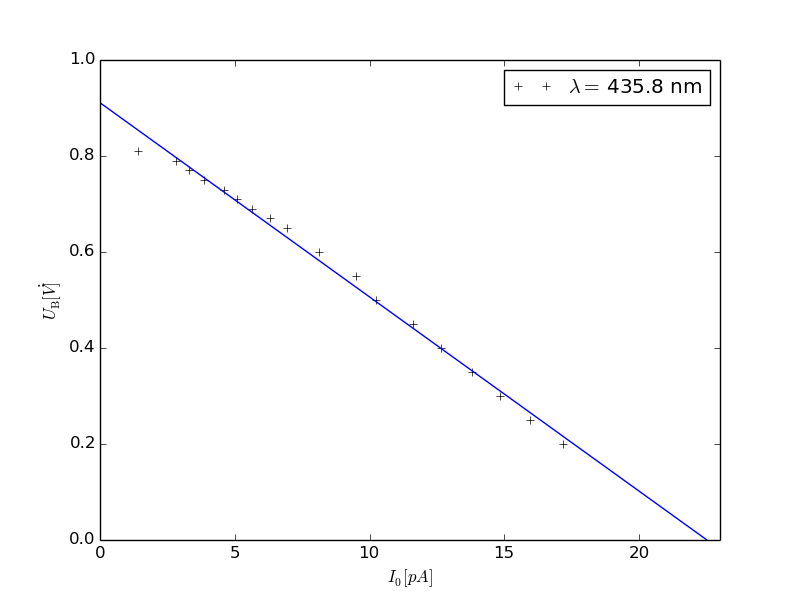
\includegraphics[width=0.75\textwidth]{Bilder/Fit_violett.png}
	\caption{Gemessene Photostromstärken in Abhängigkeit von den Bremsspannungen, Messung bei violetter Spektrallinie.}
	\label{fig:uidiagramm2}
\end{figure}
\begin{figure}[p]
	\centering
	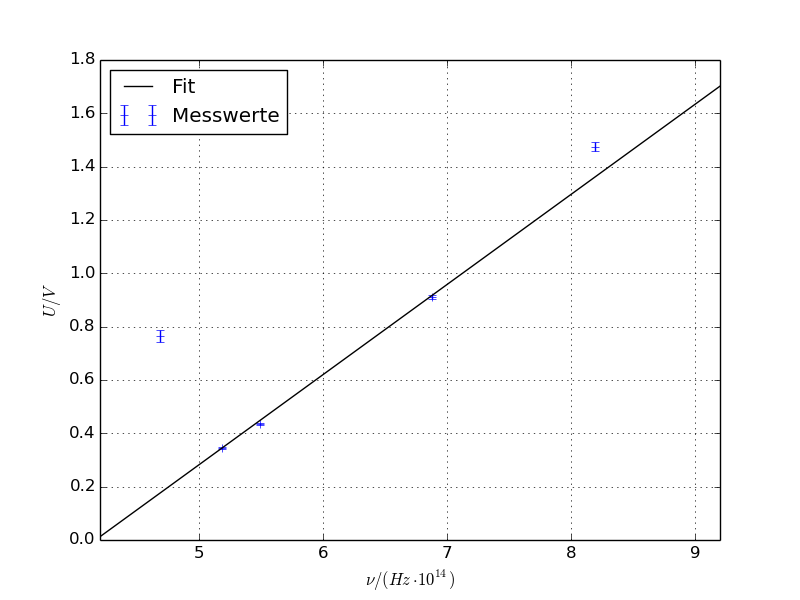
\includegraphics[width=0.85\textwidth]{Bilder/unu_diag.png}
	\caption{Maximale Bremsspannung gegen die Lichtfrequenz.}
	\label{fig:unu}
\end{figure}
\begin{landscape}
	\begin{minipage}[c][12cm][t]{0.3\textwidth}
		\centering
		\begin{tabular}{S[table-format=1.2] S[table-format=3.0]}
			\toprule
			\multicolumn{2}{c}{UV-Spektrallinie}\\ 
			\multicolumn{2}{c}{$\lambda=\SI{266.3}{\nano\meter}$}\\
			{$U_\text{B}/\:\si{\volt}$} & {$I_0/\:\si{\pico\ampere}$}\\	
			\midrule
				 0.20 & 200\\
				 0.30 & 190\\
				 0.40 & 160\\
				 0.50 & 135\\
				 0.60 & 110\\
				 0.70 &  98\\
				 0.75 &  84\\
				 0.80 &  70\\
				 0.85 &  59\\
				 0.90 &  48\\
				 0.95 &  39\\
				 1.00 &  32\\
				 1.05 &  23\\
				 1.10 &  18\\
				 1.15 &  14\\
				 1.20 &   9\\
				 1.25 &   6\\
				 1.30 &   4\\
				 1.345&   0\\
			\bottomrule
			\end{tabular}
	\end{minipage}
	\begin{minipage}[c][12cm][t]{0.3\textwidth}
		\centering
		\begin{tabular}{S[table-format=1.2] S[table-format=3.0]}
			\toprule
			\multicolumn{2}{c}{Violette Spektrallinie}\\ 
			\multicolumn{2}{c}{$\lambda=\SI{435.8}{\nano\meter}$}\\
			{$U_\text{B}/\:\si{\volt}$} & {$I_0/\:\si{\pico\ampere}$}\\	
			\midrule
				 0.20&	295\\
				 0.25&	255\\
				 0.30&	220\\
				 0.35&	190\\
				 0.40&	160\\
				 0.45&	135\\
				 0.50&	105\\
				 0.55&	 90\\
				 0.60&	 66\\
				 0.65&	 48\\
				 0.67&	 40\\
				 0.69&	 32\\
				 0.71&	 26\\
				 0.73&	 21\\
				 0.75&	 15\\
				 0.77&	 11\\
				 0.79&	  8\\
				 0.81&	  2\\
				 0.83&	  0\\
			\bottomrule
			\end{tabular}
	\end{minipage}
	\begin{minipage}[c][12cm][t]{0.3\textwidth}
		\centering
		\begin{tabular}{S[table-format=1.2] S[table-format=3.0]}
			\toprule
			\multicolumn{2}{c}{Grüne Spektrallinie}\\
			\multicolumn{2}{c}{$\lambda=\SI{546}{\nano\meter}$}\\
			{$U_\text{B}/\:\si{\volt}$} & {$I_0/\:\si{\pico\ampere}$}\\	
			\midrule
				0.10	&150\\	
				0.12	&130\\
				0.14	&120\\
				0.16	&100\\
				0.18	& 97\\
				0.20	& 81\\
				0.22	& 65\\
				0.24	& 53\\
				0.26 	& 42\\
				0.28	& 32\\
				0.30	& 25\\
				0.32	& 18\\
				0.34	& 12\\
				0.36	&  8\\
				0.38	&  4\\
				0.397	&  0\\
			\bottomrule
			\end{tabular}
	\end{minipage}
	\begin{minipage}[c][12cm][t]{0.3\textwidth}
		\centering
		\begin{tabular}{S[table-format=1.2] S[table-format=3.0]}
			\toprule
			\multicolumn{2}{c}{Gelbe Spektrallinie}\\
			\multicolumn{2}{c}{$\lambda=\SI{578}{\nano\meter}$}\\
			{$U_\text{B}/\:\si{\volt}$} & {$I_0/\:\si{\pico\ampere}$}\\	
			\midrule
				0.02	& 79\\
				0.04	& 68\\
				0.06	& 59\\
				0.08	& 50\\
				0.10	& 41\\
				0.12	& 34\\
				0.14	& 28\\
				0.16	& 22\\
				0.18	& 18\\
				0.20	& 14\\
				0.22	& 10\\
				0.24	& 8\\
				0.26	& 5\\
				0.28	& 4\\
				0.30	& 2\\
				0.32	& 0\\
			\bottomrule
			\end{tabular}
	\end{minipage}
	\begin{minipage}[c][12cm][t]{0.3\textwidth}
		\centering
		\begin{tabular}{S[table-format=1.2] S[table-format=3.0]}
			\toprule
			\multicolumn{2}{c}{Rote Spektrallinie}\\
			\multicolumn{2}{c}{$\lambda=\SI{640}{\nano\meter}$}\\
			{$U_\text{B}/\:\si{\volt}$} & {$I_0/\:\si{\pico\ampere}$}\\	
			\midrule
				0.00	&10\\
				0.05	& 8\\
				0.10	& 7\\
				0.15	& 6\\
				0.20	& 5\\
				0.25	& 4\\
				0.30	& 4\\
				0.35	& 3\\
				0.40	& 2\\
				0.45	& 2\\
				0.50	& 1\\
				0.506	& 0\\
			\bottomrule
			\end{tabular}
	\end{minipage}
\begin{table}[ht]
\caption{Die gemessenen Bremsspannungen \texorpdfstring{$U_\text{B}$}{U} und Photoströme \texorpdfstring{$I_0$}{I}in Abhängigkeit von der Wellenlänge \texorpdfstring{$\lambda$}{} des Lichtes.}
\label{tab:messwerte}
\end{table}
\end{landscape}
\subsection{Messung des Photostromes bei hohen Spannungen}

\begin{figure}[h]
	\centering
	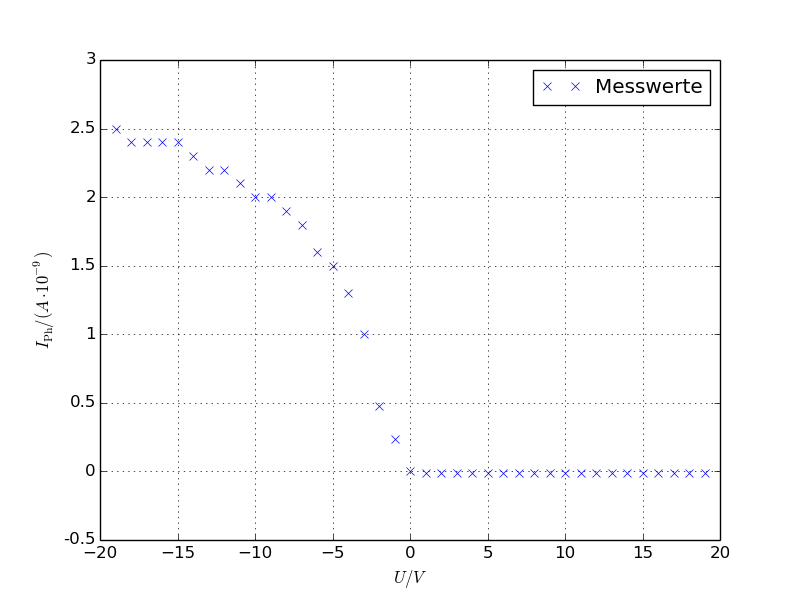
\includegraphics[width=\textwidth]{Bilder/messung2.png}
	\caption{Gemessener Photostrom in Abhängigkeit von der angelegten Spannung.}
	\label{fig:uidiagramm3}
\end{figure}
Warum erreicht die Kurve bei hohen beschleunigenden Spannungen einen Sättigungswert? 
(Widerspruch zum Ohmschen Gesetz?) 
- Kein Widerspruch
- Ohmsche Leiter übertragen Elektronen, sind aber keine Elektronenquelle,
  Photodiode stellt Elektronen zur Verfügung.

Durch welche Parameter wird der Sättigungswert festgelegt? 
- Intensität, 
- Lichtfrequenz?

Was trägt dazu bei, dass der Sättigungswert nur asymptotisch erreicht wird? 
- Photonen lösen Elektronen aus, geben ihnen dabei aber keine Richtung vor (kein Laser).
- Bei hohen Spannungen werden alle Elektronen Teil des Stromes, 
	bei geringen Spannungen werden ein Teil der Elektronen wieder absorbiert.

Wie müsste eine Photozelle konstruiert werden, bei der der Sättigungswert des Photostroms bereits bei endlichen Beschleunigungsspannungen auftritt?
- Optimales Ausnutzen der Intensität (geringe Absorption durch Glaswand, lichtdurchlässige Anode)

Warum fällt der Photostrom bei der Gegenspannung Ug nicht abrupt auf 0 ab, sondern beginnt bereits für U > Ug zu sinken?
- Ug bremst nur die schnellsten Elektronen ab, der Großteil der Elektronen sind bereits bei kleineren Spannungen abgebremst.

Warum kann ein dem Photostrom entgegengerichteter Strom auftreten? 
(Hinweis: Die Photokathode besteht aus einem Material, das bereits bei T = 20°C merklich verdampft.) 
- 

Warum kann hier bereits bei relativ kleinen Spannungsbeträgen praktisch ein Sättigungswert erreicht werden?
- Die Intensität scheint groß zu sein

Was kann man über die Austrittsarbeit der Anode sagen, wenn man berücksichtigt, dass der negative Strom bereits bei der
Einstrahlung energiearmen Lichtes (λ etwa 650nm) auftritt? 
- Austrittsarbeit ist gering.